\cotefile{57}
\scanpage{150}\mspage{40}
Now let $V$ be a compact analytic surface with two algebraically independent meromorphic functions $x$, $y$. Then, by the result of Chow mentioned above, $\unsure{\mathfrak{M}|\mathscr{M}}(V)$ is a finite algebraic extension of the field $\unsure{\mathfrak{C}|\mathbb{C}}(x,y)$ of rational functions in $x$, $y$. (A proof of this fact based on our results in Section 1 will be given in Appendix below.) Hence there exists a \uuline{non-singular} al\uline{gebraic surf}ace $V^{*}$ in a projective space such that $\mathfrak{M}(V)\cong\mathfrak{M}(V^{*})$. Letting $(1,x_{1}^{*},\cdots,x_{d}^{*})$ be the \uline{generic} point of $V^{*}$ and letting $x_{k}=x_{k}(z)$ be the meromorphic function on $V$ corresponding to $x_{k}^{*}$ by the isomorphism $\mathfrak{M}(V)\cong\mathfrak{M}(V^{*})$, we define a meromorphic mapping $\Phi$ of $V$ onto $V^{*}$ by
\[
z\longrightarrow\Phi(z)=(1,x_{1}(z),\cdots,x_{d}(z)).
\]
This mapping $\Phi$ is regular on $V$ except for a finite number of its fundamental points. These fundamental points can be eliminated by means of quadratic transformations. Namely, by applying a finite number of suitable quadratic transformations $Q_{\mathfrak{p}}, Q_{\mathfrak{p}'}, Q_{\mathfrak{p}''},\cdots$ to $V$ successively, we obtain a compact analytic surface
\[
\widetilde{V}=\cdot\cdot\cdot\cdot\, Q_{\mathfrak{p}''}Q_{\mathfrak{p}'}Q_{\mathfrak{p}}(V)
\]
such that the mapping $\widetilde{\Phi}=\Phi\,Q_{\mathfrak{p}}^{-1}Q_{\mathfrak{p}'}^{-1}Q_{\mathfrak{p}''}^{-1}\cdots$ of $\widetilde{V}$ onto $V^{*}$ is everywhere regular.\footnotemark[7] Since $\Phi$ induces the isomorphism
\footnotetext[7]{Chow and Kodaira, loc. cit., p. 322.}
% archive sheet number: 149
\scanpage{151}
\deleted{il \unsure{paraît|faut} \unsure{évident|en effet}} les $C_i$ sont non \unsure{singuliers|singulières} [car $\operatorname{Pic}^{0}_{C_i/k}\deleted{\unsure{C|k}}$ est un quotient de $\operatorname{Pic}^{0}_{C/k}$] et que \deleted{\unsure{aux|Alors} $\unsure{P'_{\alpha}|P_{\alpha}|\mu'_{\alpha}}$ \unsure{où les} \unsure{$\nu_{\alpha}$} \inserted{$\nu_{\alpha}$} $C_i$ \unsure{passent par un même pt}} \unsure{que|pour|On a} si $i\ne j$, alors $C_i$ et $C_j$ se \unsure{coupent} en un pt au plus [car $\operatorname{Pic}(C_i\cup C_j)$ est un quotient de $\operatorname{Pic}(C)$]. \deleted{\unsure{Soit} $\nu_{\alpha}$ le nb des $C_i$ \unsure{passant par} $P_{\alpha}$, on a}
\[
\begin{aligned}
\dim G_{\mathrm{mult}}&=\sum(\nu_{\alpha}-1)-c_{0}+1\\
 &=\sum_{i}(\text{\unsure{nbre|nb} de pts }P_{\alpha}\text{ sur } C_i-1)-
\end{aligned}
\]
\unsure{Plus|D'ailleurs} \unsure{précisément|généralement}, on \unsure{trouve|trouvera} de cette façon que l'on ne peut avoir de cycles
\figure{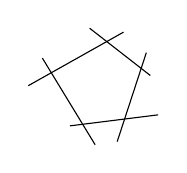
\begin{tikzpicture}[x=1cm,y=1cm]
\draw (-.22,.61)--(.99,1.29);
\draw (-.04,.96)--(.63,-.14);
\draw (.56,1.34)--(1.33,.74);
\draw (1.28,1.03)--(.91,-.10);
\draw (.31,.10)--(1.43,.24);
\end{tikzpicture}}
dans le \unsure{schéma} combinatoire de $C$. \deleted{\unsure{C'est suffisant},} \unsure{Réciproquemt|Réciproquement}, si $C$ n'a pas de pts \deleted{\unsure{doubles}} \inserted{multiples} ``multiplicatifs'', et si \deleted{\unsure{tous|les}} $C_i$ sont non \unsure{singuliers|singulières}, on voit par récurrence sur le nb des $C_i$ que $C$ \deleted{\unsure{est|$\to$}} $\operatorname{Pic}^{0}_{C/k}$ est une V.A.

On aura en tous cas
\margin{$g_i=\text{genre de }\widetilde{C}_i$}
\[
\begin{aligned}
g=\dim\operatorname{Pic}_{C/k}&=\sum g_i+\left(\sum_{\alpha}\mu_{\alpha}-c_{0}+1\right)\\
 &=\sum g_i+\deleted{\unsure{\mu_{\alpha}|\nu_{\alpha}}}\rho+\sigma
\end{aligned}
\]
$\rho=$ nb des cycles combinatoires, $+$ \unsure{somme|nombre} des \unsure{ints|ints.} des \unsure{multiplicités|multiplications} multiplicatives des $C_i$ [\unsure{cette} \unsure{dernière} $0$ si les $C_i$ non sing.]

$\sigma=$ somme des multiplicités additives des $P_{\alpha}$.
% archive sheet number: 150
\scanpage{152}\mspage{39}
regular map of $\widetilde{V}$ onto $V$ which is bi-regular between $\widetilde{V}-S$ and $V-\mathfrak{p}$. It is easy to prove the following propositions:\footnotemark[4]

i) $Q_{\mathfrak{p}}^{-1}$ induces an isomorphism: $\unsure{\mathfrak{M}|\mathscr{M}}(Q_{\mathfrak{p}}(V))\cong\mathfrak{M}(V)$.

ii) If $V$ is a non-singular algebraic surface in a projective space, then $Q_{\mathfrak{p}}(V)$ is also a non-singular algebraic surface in a projective space.

Moreover we have

\begin{quote}
CASTELNUOVO-ENRIQUES' THEOREM:\footnotemark[5] Let $\widetilde{V}$ be a non-singular algebraic surface in a projective space and let $S$ be a non-singular rational curve on $\widetilde{V}$ with $(S^{2})=-1$. Then there exists a non-singular algebraic surface $V$ in a projective space and a point $\mathfrak{p}$ on $V$ such that $Q_{\mathfrak{p}}(V)=\widetilde{V}$ and $Q_{\mathfrak{p}}(\mathfrak{p})=S$.
\end{quote}

The following proposition\footnotemark[6] is a corollary to this theorem:

iii) If $Q_{\mathfrak{p}}(V)$ is a non-singular algebraic surface in a projective space, then $V$ is also a non-singular algebraic surface in a projective space.
\footnotetext[4]{See Chow and Kodaira, loc. cit.}
\footnotetext[5]{G. Castelnuovo and F. Enriques, Sopra alcune questioni fondamentali nella teoria delle superficie algebriche, Annali di Math., Ser. III, Vol. 6 (1901), pp. 165-225, Chap. III. See also K. Kodaira, On Kähler varieties of restricted type, Annals of Math., Vol. 60 (1954), pp. 44-48.}
\footnotetext[6]{Chow and Kodaira, loc. cit., Lemma 3.}
% archive sheet number: 151
\scanpage{153}
\figure{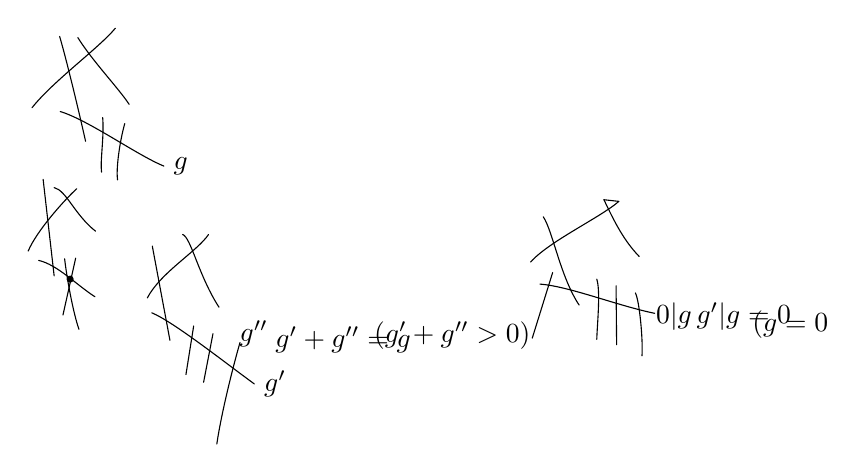
\begin{tikzpicture}[x=.007cm,y=-.007cm,line cap=round]
\draw (196,340).. controls (235,291) and (316,233)..(347,196);
\draw (246,211).. controls (260,259) and (282,352)..(293,401);
\draw (279,213).. controls (305,255) and (353,305)..(372,334);
\draw (247,347).. controls (299,363) and (386,426)..(435,446) node[right] {$g$};
\draw (324,358).. controls (327,392) and (319,438)..(322,457);
\draw (364,369).. controls (355,401) and (348,450)..(351,471);
\draw (189,600).. controls (204,564) and (254,508)..(277,487);
\draw (216,470)--(236,645);
\draw (236,485).. controls (258,490) and (273,534)..(311,564);
\draw (208,617).. controls (242,625) and (276,661)..(310,683);
\draw (255,614).. controls (259,650) and (271,714)..(281,742);
\draw (275,613)--(252,716);
\fill (265,651) circle[radius=.045cm];
\draw (405,685).. controls (429,639) and (495,601)..(516,570);
\draw (414,591)--(446,762);
\draw (469,570).. controls (484,575) and (498,645)..(535,702);
\draw (413,712).. controls (452,728) and (548,804)..(599,841) node[right] {$g'$};
\draw (489,736)--(475,824); \draw (524,750)--(507,838);
\draw (573,766).. controls (560,811) and (539,895)..(531,950);
\node at (598,750) {$g''$};
\node at (760,761) {$g'+g''=g$};
\node at (958,754) {$(g'+g''>0)$};
\draw (1100,620).. controls (1134,582) and (1227,539)..(1260,510);
\draw (1123,538).. controls (1140,563) and (1154,647)..(1188,698);
\draw (1233,507).. controls (1252,547) and (1269,581)..(1297,610);
\draw (1233,507)--(1260,510);
\draw (1117,660).. controls (1170,664) and (1257,699)..(1325,713);
\draw (1140,639)--(1103,758);
\draw (1220,651).. controls (1227,673) and (1221,730)..(1220,760);
\draw (1255,663)--(1256,770);
\draw (1290,676).. controls (1297,689) and (1304,758)..(1302,790);
\node[anchor=west] at (1310,719) {$\deleted{\unsure{0|g}}\,\unsure{g'|g}=0$};
\node at (1571,733) {$(g=0$};
\end{tikzpicture}}
\[
\sum_{g_i\geq1}(3g_i-3+\nu_i\deleted{\unsure{-1|1}})
+\sum_{g_i=1}(1\underbrace{+\nu_i-1}_{3g_i-3+\nu_i})
+\sum_{\substack{g_i=0\\\nu_i\geq3}}\deleted{\unsure{\substack{\sup(0,\\\sup(0,}}}\underset{3g_i-3+\nu_i}{\nu_i-3}
\]
$\nu_i=$ nb des pts \deleted{\unsure{multiples}} \inserted{\unsure{$P_{\alpha}$|dbls|doubles}} sur $C_i$
\[
3\sum g_i-3c_0+\sum\nu_i\overset{\inserted{\lambda}}{+}
\boxed{\sum_{\substack{g_i=0\\\nu_i\unsure{\leq|=}2}}3-\nu_i}
\]
$\lambda=$ nb des \deleted{\unsure{courbes|composantes}} $C_i$ de genre $0$, avec $\nu_i=2$ (\unsure{minimum})

\figure{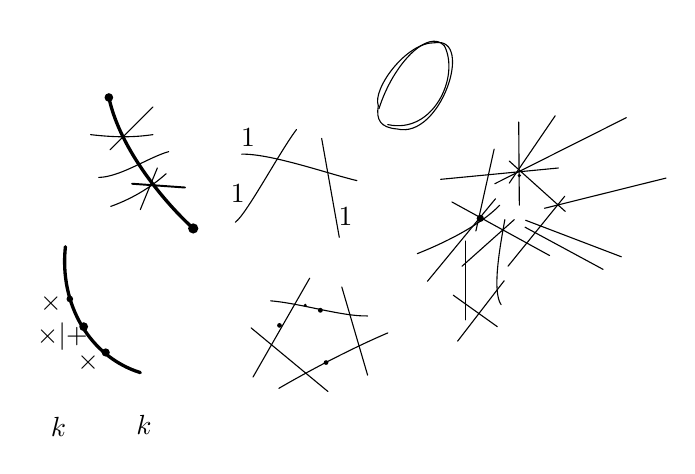
\begin{tikzpicture}[x=.008cm,y=-.008cm,line cap=round]
\draw (649,1454).. controls (639,1428) and (693,1353)..(739,1354)
.. controls (802,1344) and (748,1508)..(679,1491).. controls (653,1489) and (645,1477)..(649,1454);
\draw (650,1459).. controls (673,1386) and (729,1331)..(754,1359)
.. controls (779,1408) and (736,1500)..(664,1484);
\draw[line width=1.2pt] (221,1441).. controls (239,1525) and (312,1610)..(355,1649);
\fill (221,1441) circle[radius=.055cm]; \fill (355,1649) circle[radius=.065cm];
\draw (192,1500).. controls (235,1505) and (263,1504)..(291,1500);
\draw (223,1524)--(291,1456);
\draw (205,1568).. controls (240,1567) and (284,1536)..(316,1527);
\draw (224,1614).. controls (263,1600) and (292,1580)..(312,1562);
\draw[line width=.7pt] (258,1578)--(342,1584); \draw (271,1619)--(298,1553);
\draw (422,1639).. controls (440,1626) and (493,1526)..(519,1492);
\draw (432,1531).. controls (479,1530) and (572,1563)..(615,1573);
\draw (559,1506)--(587,1663);
\node at (442,1504) {$1$}; \node at (426,1593) {$1$}; \node at (597,1630) {$1$};
\draw[line width=1.2pt] (152,1678).. controls (142,1770) and (191,1853)..(271,1878);
\fill (159,1761) circle[radius=.042cm]; \fill (181,1805) circle[radius=.056cm]; \fill (216,1846) circle[radius=.052cm];
\node at (129,1768) {$\times$}; \node at (147,1820) {$\unsure{\times|+}$}; \node at (188,1862) {$\times$};
\node at (141,1964) {$k$}; \node at (277,1961) {$k$};
\draw (478,1764).. controls (526,1768) and (592,1789)..(632,1788);
\draw (450,1885)--(540,1728); \draw (591,1742)--(632,1882);
\draw (447,1807)--(569,1908);
\draw (491,1903).. controls (546,1871) and (610,1838)..(664,1815);
\fill (492,1803) circle[radius=.03cm]; \fill (533,1771) circle[radius=.021cm];
\fill (557,1779) circle[radius=.031cm]; \fill (566,1862) circle[radius=.03cm];
\draw (748,1571)--(935,1553); \draw (872,1480)--(873,1612);
\draw (834,1578)--(1043,1473); \draw (857,1577)--(930,1470);
\draw (857,1542)--(946,1622); \draw (913,1617)--(1106,1569);
\draw (833,1523)--(804,1653); \draw (711,1689).. controls (754,1672) and (811,1644)..(842,1612);
\draw (766,1607)--(921,1692); \draw (727,1733)--(835,1602);
\draw (782,1709)--(865,1635); \draw (850,1635).. controls (841,1684) and (830,1749)..(844,1770);
\draw (855,1709)--(945,1598); \draw (883,1636)--(1035,1694); \draw (882,1647)--(1006,1714);
\draw (788,1669)--(788,1794); \draw (768,1755)--(838,1805); \draw (775,1828)--(849,1732);
\fill (811,1633) circle[radius=.046cm]; \fill (873,1565) circle[radius=.023cm];
\end{tikzpicture}}
\margin{[tout cycle est formé \unsure{exclusivemt|exclusivement} de courbes rationnelles, et \deleted{\unsure{est de longueur}} \inserted{\unsure{un cycle}} minimum est de longueur \unsure{au|n}}%
\[
\sum g_i=g-\overset{\substack{\text{\unsure{nb des cycles}}\\\text{\unsure{combin.|combinatoires}}}}{\rho}.
\]
\[
3g-
\]
% archive sheet number: 152
\scanpage{154}
% margin note written sideways
\margin{\textbf{Imp.\quad A. GROTHENDIECK.---Publications mathématiques, n\textsuperscript{o} 4.\\ P. U. F.\quad Placard 36}}

\textit{Proposition} \textbf{(6.4.12)}. --- \textit{Soient $f:\mathrm{X}\to \mathrm{Y}$, $g:\mathrm{Y}'\to \mathrm{Y}$ deux morphismes\,; posons $\mathrm{X}'=\mathrm{X}\times_{\mathrm{Y}}\mathrm{Y}'$ et soit $f'=f_{(\mathrm{Y}')}:\mathrm{X}'\to \mathrm{Y}'$. Soit $y'\in \mathrm{Y}'$, $y=g(y')$\,; si la fibre $f^{-1}(y)$ est un schéma algébrique fini sur $\varkappa(y)$, alors la fibre ${f'}^{-1}(y')$ est un schéma algébrique fini sur $\varkappa(y')$, ayant même rang et même nombre géométrique de points que $f^{-1}(y)$.}

Compte tenu de la transitivité des fibres (3.6.5), cela résulte aussitôt de (6.4.6) et (6.4.8).

\textbf{(6.4.13)} La prop. (6.4.11) montre que les morphismes de type fini correspondent intuitivement aux « familles algébriques de variétés algébriques », les points de $\mathrm{Y}$ jouant le rôle de « paramètres »\,; ce \deleted{sont donc les seuls} \inserted{\handwritten{qui donne à ces}} morphismes \deleted{qui aient} une signification « géométrique ». \margin{\handwritten{$\times$}} Les morphismes qui ne sont pas de type fini interviendront surtout par la suite dans les questions de « changement du préschéma de base », par exemple par localisation ou complétion.

\textbf{6.5. Détermination locale d’un morphisme.}

\textit{Proposition} \textbf{(6.5.1)}. --- \textit{Soient $\mathrm{X}$, $\mathrm{Y}$ deux $\mathrm{S}$-préschémas, $\mathrm{Y}$ étant de type fini sur $\mathrm{S}$\,; soient $x\in \mathrm{X}$, $y\in \mathrm{Y}$ au-dessus d’un même point $s\in \mathrm{S}$.}

(i) \textit{Si deux $\mathrm{S}$-morphismes $f=(\psi,\theta)$, $f'=(\psi',\theta')$ de $\mathrm{X}$ dans $\mathrm{Y}$ sont tels que $\psi(x)=\psi'(x)=y$, et que les $\mathcal{O}_s$-homomorphismes (locaux) $\theta_x^{\sharp}$ et ${\theta'}^{\sharp}_x$ de $\mathcal{O}_y$ dans $\mathcal{O}_x$ soient identiques, $f$ et $f'$ coïncident dans un voisinage ouvert de $x$.}

(ii) \textit{Supposons en outre $\mathrm{S}$ localement noethérien. Pour tout $\mathcal{O}_s$-homomorphisme local $\varphi:\mathcal{O}_y\to\mathcal{O}_x$, il existe un voisinage ouvert $\mathrm{U}$ de $x$ dans $\mathrm{X}$ et un $\mathrm{S}$-morphisme $f=(\psi,\theta)$ de $\mathrm{U}$ dans $\mathrm{Y}$ tels que $\psi(x)=y$ et $\theta_x^{\sharp}=\varphi$.}

(i) La question étant locale sur $\mathrm{S}$, $\mathrm{X}$ et $\mathrm{Y}$, on peut supposer $\mathrm{S}$, $\mathrm{X}$, $\mathrm{Y}$ affines d’anneaux respectifs $\mathrm{A}$, $\mathrm{B}$, $\mathrm{C}$, $f$ et $f'$ étant de la forme $({}^{a}\varphi,\widetilde{\varphi})$ et $({}^{a}\varphi',\widetilde{\varphi}')$ respectivement, où $\varphi$ et $\varphi'$ sont deux $\mathrm{A}$-homomorphismes de $\mathrm{C}$ dans $\mathrm{B}$ tels que $\varphi^{-1}(\unsure{\mathfrak{j}|\mathrm{j}}_x)={\varphi'}^{-1}(\mathfrak{j}_x)=\mathfrak{j}_y$, et les homomorphismes $\varphi_x$ et $\varphi'_x$ de $\mathrm{C}_y$ dans $\mathrm{B}_x$, déduits de $\varphi$ et $\varphi'$, sont identiques\,; on peut en outre supposer que $\mathrm{C}$ est une $\mathrm{A}$-algèbre \textit{de type fini}. Soient $c_i$ $(1\leqslant i\leqslant n)$ des générateurs de la $\mathrm{A}$-algèbre $\mathrm{C}$, et posons $b_i=\varphi(c_i)$, $b'_i=\varphi'(c_i)$\,; par hypothèse, on a $b_i/1=b'_i/1$ dans l’anneau de fractions $\mathrm{B}_x$ $(1\leqslant i\leqslant n)$. Cela signifie qu’il existe des éléments $s_i\in \mathrm{B}-\mathfrak{j}_x$ tels que $s_i(b_i-b'_i)=0$ pour $1\leqslant i\leqslant n$, et on peut évidemment supposer tous les $s_i$ égaux à un même élément $g\in \mathrm{B}-\mathfrak{j}_x$. On en conclut que l’on a $b_i/1=b'_i/1$ pour $1\leqslant i\leqslant n$ dans l’anneau de fractions $\mathrm{B}_g$\,; si $i_g$ est l’homomorphisme canonique $\mathrm{B}\to \mathrm{B}_g$, on a par suite $i_g\circ\varphi=i_g\circ\varphi'$\,; donc les restrictions de $f$ et $f'$ à $\mathrm{D}(g)$ sont identiques.

(ii) On peut se ramener à la même situation que dans (i), et supposer en outre que l’anneau $\mathrm{A}$ est \textit{noethérien}. Soient $c_i$ $(1\leqslant i\leqslant n)$ des générateurs de la $\mathrm{A}$-algèbre $\mathrm{C}$, et soit $\alpha:\mathrm{A}[\mathrm{X}_1,\ldots,\mathrm{X}_{\unsure{n|i}}]\to \mathrm{C}$ l’homomorphisme de l’algèbre de polynômes $\mathrm{A}[\mathrm{X}_1,\ldots,\mathrm{X}_n]$ sur $\mathrm{C}$ transformant $\mathrm{X}_i$ en $c_i$ pour $1\leqslant i\leqslant n$. Soit d’autre part $i_y$ l’homomorphisme canonique $\mathrm{C}\to \mathrm{C}_y$, et considérons l’homomorphisme composé
\[
\beta:\mathrm{A}[\mathrm{X}_1,\ldots,\mathrm{X}_n]\xrightarrow{\alpha}\mathrm{C}\xrightarrow{\unsure{iy|i_y}}\mathrm{C}_y\xrightarrow{\varphi}\mathrm{B}_x.
\]
% archive sheet number: 153
\scanpage{155}
\[
\text{Conditions équivalentes :}\quad
\left\{\begin{aligned}
&\text{a) }\operatorname{Pic}^{0}_{C/k}\text{ est \unsure{abélien}}\\
&\text{b) les }\unsure{\kappa_{\alpha}|\mu_{\alpha}}=0\ \text{i.e. tous les pts doubles sont ordinaires,}\\
&\qquad\text{\uuline{et} }b_1=0\quad\text{[En particulier les }C_i\text{ sont non \unsure{singulières|singuliers}]}
\end{aligned}\right.
\]
\[
\text{Conditions équivalentes}\quad
\left\{\begin{aligned}
&\text{a) }\operatorname{Pic}^{0}_{C/k}\ \text{\unsure{n'a} pas de \unsure{composante} additive}\\
&\text{b) \deleted{\unsure{Pour|Donc}} }\unsure{\forall|\text{tt}}\,\alpha,\ \text{on a }\mu_{\alpha}=\unsure{\mu'_{\alpha}|\kappa'_{\alpha}}\\
&\qquad\text{i.e. le \unsure{recollement|conducteur} est trivial.}
\end{aligned}\right.
\]
\figure{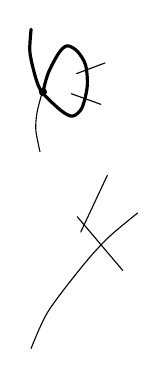
\begin{tikzpicture}[x=.0075cm,y=-.0075cm,line cap=round,line join=round]
\draw[line width=1.15pt] plot[smooth] coordinates {(84,518) (82,557) (92,601) (103,625) (134,655) (154,665) (170,651) (179,614) (176,578) (162,555) (145,546) (131,558) (113,592) (104,624)};
\draw plot[smooth] coordinates {(103,624) (94,659) (92,689) (99,725)};
\draw (161,593)--(209,575);
\draw (152,627)--(202,645);
\fill (104,624) circle[radius=.052cm];
\draw plot[smooth] coordinates {(84,1058) (113,995) (173,916) (215,870) (264,829)};
\draw (162,835)--(239,926);
\draw (168,861)--(213,765);
\end{tikzpicture}}
\[
\sum_i\nu_i=\underset{\mu_{\alpha}-1}{\sum_{\alpha}(\mu_{\alpha})}\deleted{\unsure{+1)|+1}}
=\underbrace{\sum_{\unsure{\beta|\rho}}(\deleted{\unsure{+}}\mu_{\alpha}-1)}_{c_0-1+\rho}+c_1
\]
\[
\deleted{\unsure{g=|g|\substack{3\\6}}}\qquad
\boxed{\sum\nu_i=c_0-1+\rho+c_1}
\]
\margin{$\rho=g-\sum g_i$\par $\sum g_i=g-\rho$}
\[
\begin{aligned}
&3g-\underbrace{3\rho-3c_0+\deleted{c_0}-1+\rho}{}+c_1+\lambda\\
&3g-2\rho-2c_0+c_1+\lambda-1\\
&3g-3\quad \deleted{\unsure{=2c|=2}}\,[2(c_0+\rho)-c_1-\lambda-2]
\end{aligned}
\]
\figure{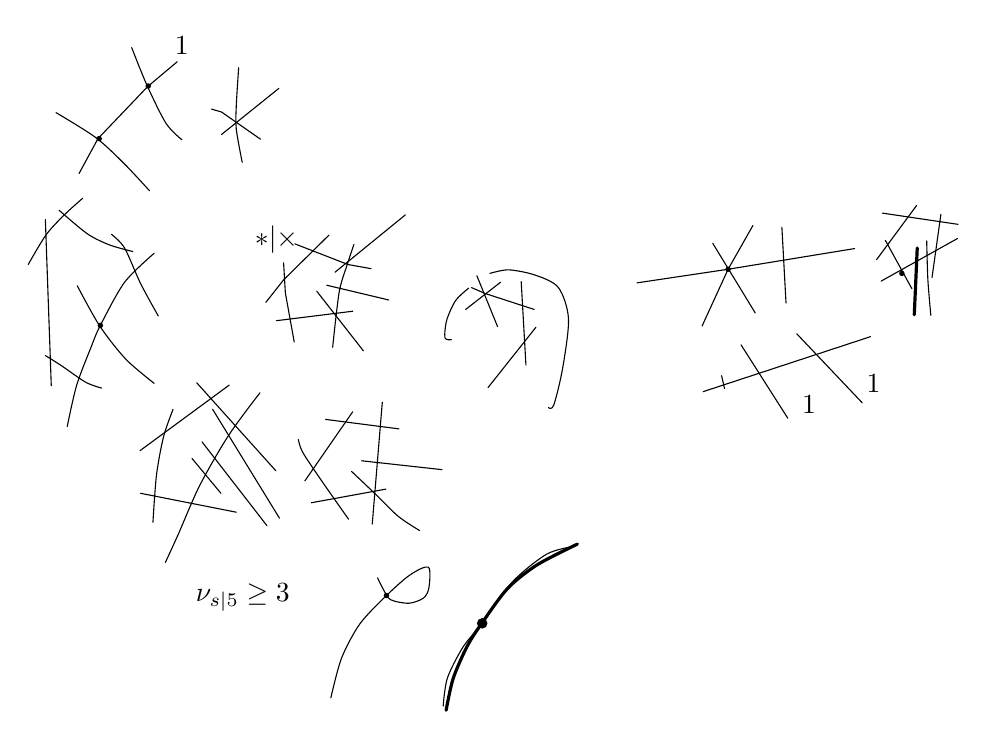
\begin{tikzpicture}[x=.0075cm,y=-.0075cm,line cap=round,line join=round]
\draw (144,1280)--(176,1221)--(260,1133)--(310,1091);
\draw plot[smooth] coordinates {(105,1177) (172,1219) (220,1263) (263,1309)};
\draw plot[smooth] coordinates {(233,1067) (259,1131) (291,1195) (318,1223)};
\node at (318,1064) {$1$};
\fill (178,1221) circle[radius=.035cm];
\fill (261,1132) circle[radius=.035cm];
\draw (368,1171)--(385,1176)--(451,1222);
\draw plot[smooth] coordinates {(414,1101) (410,1165) (410,1205) (420,1261)};
\draw (385,1214)--(482,1136);
\draw plot[smooth] coordinates {(58,1434) (88,1384) (119,1350) (150,1322)};
\draw plot[smooth] coordinates {(110,1342) (158,1382) (196,1401) (235,1412)};
\draw (87,1358)--(97,1639);
\draw plot[smooth] coordinates {(199,1383) (221,1406) (248,1466) (278,1521)};
\draw plot[smooth] coordinates {(124,1708) (140,1638) (165,1572) (180,1537) (221,1464) (271,1415)};
\draw plot[smooth] coordinates {(141,1470) (179,1538) (223,1594) (271,1635)};
\draw plot[smooth] coordinates {(87,1588) (114,1605) (155,1633) (182,1643)};
\fill (180,1537) circle[radius=.035cm];
\draw (460,1498)--(490,1460)--(567,1384);
\draw (490,1431)--(493,1482)--(508,1565);
\draw (509,1399)--(599,1434)--(638,1441);
\draw (577,1447)--(696,1350);
\draw plot[smooth] coordinates {(609,1400) (597,1436) (584,1481) (573,1574)};
\draw (563,1469)--(668,1494);
\draw (546,1479)--(625,1580);
\draw (478,1529)--(607,1513);
\node at (478,1392) {$\unsure{*|\times}$};
\draw plot[smooth] coordinates {(774,1561) (763,1558) (766,1528) (781,1495) (803,1474)};
\draw plot[smooth] coordinates {(839,1449) (871,1443) (916,1452) (955,1473) (972,1526) (962,1610) (947,1672) (938,1676)};
\draw (808,1473)--(831,1483)--(914,1510);
\draw (817,1453)--(852,1539);
\draw (798,1510)--(857,1464);
\draw (892,1463)--(900,1604);
\draw (836,1642)--(917,1540);
\draw (1088,1465)--(1242,1442)--(1456,1407);
\draw (1198,1538)--(1242,1442)--(1284,1368);
\draw (1216,1398)--(1288,1516);
\draw (1333,1371)--(1340,1499);
\fill (1242,1442) circle[radius=.035cm];
\draw (1493,1426)--(1561,1334);
\draw (1503,1347)--(1631,1366);
\draw (1508,1393)--(1553,1475);
\draw (1501,1462)--(1630,1390);
\draw (1602,1349)--(1587,1456);
\draw[line width=1.15pt] (1562,1406)--(1557,1519);
\draw plot[smooth] coordinates {(1578,1394) (1580,1460) (1585,1520)};
\fill (1536,1449) circle[radius=.035cm];
\draw (1200,1649)--(1483,1556);
\draw (1264,1570)--(1343,1694);
\draw (1358,1551)--(1469,1668);
\draw (1231,1622)--(1236,1644);
\node at (1379,1671) {$1$};
\node at (1488,1635) {$1$};
\draw (247,1749)--(398,1638);
\draw plot[smooth] coordinates {(269,1870) (275,1790) (287,1725) (303,1679)};
\draw (248,1821)--(410,1853);
\draw plot[smooth] coordinates {(290,1938) (312,1890) (348,1808) (397,1723) (450,1651)};
\draw (343,1634)--(477,1783);
\draw (370,1679)--(483,1863);
\draw (352,1734)--(462,1876);
\draw (335,1762)--(384,1821);
\draw (526,1800)--(607,1683);
\draw plot[smooth] coordinates {(515,1730) (522,1751) (551,1795) (600,1865)};
\draw (561,1696)--(685,1712);
\draw (657,1667)--(640,1873);
\draw (622,1766)--(758,1781);
\draw (537,1837)--(663,1814);
\draw plot[smooth] coordinates {(605,1784) (645,1822) (684,1860) (720,1884)};
\node at (421,1997) {$\nu_{\unsure{s|5}}\geq3$};
\draw plot[smooth] coordinates {(570,2167) (588,2100) (619,2042) (664,1994) (704,1959) (735,1946) (736,1980) (727,1998) (702,2007) (671,2001) (659,1984) (649,1964)};
\fill (664,1994) circle[radius=.035cm];
\draw[line width=1.15pt] plot[smooth] coordinates {(765,2188) (777,2134) (801,2079) (826,2040) (869,1982) (919,1942) (987,1907)};
\draw plot[smooth] coordinates {(760,2181) (767,2134) (793,2082) (824,2043) (877,1971) (935,1924) (980,1911)};
\fill (826,2041) circle[radius=.067cm];
\end{tikzpicture}}
Courbe elliptique $+k$ points dessus $(k\geq1)$.
\[
\unsure{k|R},\qquad 9-5=4
\]
\[
-6+2-1=-5
\]
% archive sheet number: 154
\scanpage{156}\mspage{41}
$\unsure{\mathfrak{M}|\mathscr{M}}(V)\cong\mathfrak{M}(V^{*})$, we infer from the proposition i) that $\widetilde{\Phi}$ induces an isomorphism $\mathfrak{M}(\widetilde{V})\cong\mathfrak{M}(V^{*})$.

The inverse mapping $\widetilde{\Phi}^{-1}$ has possibly a finite number of fundamental points and branch curves and, except for these \uline{singular points}, $\widetilde{\Phi}^{-1}$ is locally bi-regular. Hence, for any general point $\mathfrak{p}^{*}$ on $V^{*}$, the inverse image $\widetilde{\Phi}^{-1}(\mathfrak{p}^{*})$ consists of a finite number of points and the number $m$ of these points is independent of $\mathfrak{p}^{*}$. Now we show that $m=1$. Let $D_h^{*}$ be the section of $V^{*}$ cut out by a general hypersurface of order $h$ containing no fundamental point of $\widetilde{\Phi}^{-1}$ and set $D_h=\widetilde{\Phi}^{-1}(D_h^{*})$. Then, since $\widetilde{\Phi}$ induces the isomorphism $\mathfrak{M}(\widetilde{V})\cong\mathfrak{M}(V^{*})$, \uline{the complete linear system} $\lvert D_h\rvert$ \uline{on} $\widetilde{V}$ \uline{and the complete linear system} $\lvert D_h^{*}\rvert$ \uline{on} $V^{*}$ \uline{have the same diemsion}. For sufficiently large $h$, we infer from the theorem of Riemann-Roch (2.10) and Theorem 2.4 that
\[
\dim\lvert D_h^{*}\rvert=\frac{1}{2}(D_h^{*2})-\frac{1}{2}(K^{*}D_h^{*})+\chi(V^{*})-1,
\]
where $K^{*}$ is the canonical bundle on $V^{*}$. Setting $2a=(D_1^{*2})$, $2b^{*}=(K^{*}D_1^{*})$, we get therefore
\[
\dim\lvert D_h^{*}\rvert=ah^2-b^{*}h+\chi(V^{*})-1.
\]
On the other hand, we get, using (2.10),
\[
\dim\lvert D_h\rvert\geqq\frac{1}{2}(D_h^{2})-\frac{1}{2}(KD_h)+\chi(\widetilde{V})-1-i(D_h).
\]
The general member $D_h^{*}$ of $\lvert D_h^{*}\rvert$ is an irreducible non-singular curve on $V^{*}$. Let $D_h^{*\prime}$ be another general member of $\lvert D_h^{*}\rvert$ and
% archive sheet number: 155
\scanpage{157}
\begin{flushright}
\unsure{Foncteur|Foncteurs} de Picard,\\
Diviseurs \ldots
\end{flushright}
% archive sheet number: 156
\scanpage{158}
$X$ schéma \uline{\unsure{Steinien}} sur $S$

\deleted{\illegible{1}} Soit $\underline{L}$ inversible \inserted{très ample} sur $X$, tel que $f_{*}(\underline{L})\inserted{=E}$ [loc. libre de rang $N$] \inserted{tel que} $i:X\to P(\deleted{\unsure{f_{*}\underline{L}}}E)$ soit défini.
% slanted
\margin{\unsure{inutile} ?}

A) Équivalence

(i) Donner une base de $E=f_{*}(\underline{L})$ i.e. un \uline{isom} $\underline{O}_{S}^{N}\xrightarrow{\sim}\deleted{\unsure{f_{*}(\underline{L})|E}}E$

(ii) Donner un isom $\varphi:P_{S}^{N}\xrightarrow{\sim}P(\deleted{\unsure{f_{*}\underline{L}}}E)$, $\oplus$ un isom $(\varphi^{-1}i)^{*}(\underline{O}(1))\simeq\underline{L}$

(iii) Donner un \deleted{\unsure{isomorphisme|isom}} morphisme
\[
j:X\longrightarrow P_{S}^{N}
\]
$\oplus$ un isomorphisme $\alpha:j^{*}(\underline{O}(1))\simeq\underline{L}$
% slanted
\margin{\unsure{Lors|Pour|Dans} la définition des \unsure{équival\textsuperscript{ces}|équival\textsuperscript{ts}|équivalence}, faire attention qu'on exige que le changement de base le conserve \deleted{\uuline{\unsure{Non|N.B.}}, puisque on fait cette hypothèse \unsure{dans} \unsure{l'un|d'un} \unsure{indépendant|indépen\textsuperscript{t}}} \inserted{\uline{morphisme spécial}}}
tels que l'hom correspondant
\[
g_{*}\underline{O}(1)\longrightarrow f_{*}(\underline{L})=E
\]
soit un isom. [condition qui ne dépend pas du choix de $\alpha$]
\margin{Compatibilité aux opérations de $\unsure{\operatorname{GL}(N)|\operatorname{Gl}|\Gamma(\underline{O}_{S}^{*})}$ et localisation.}

A') Équivalence

(i) Donner une \deleted{\unsure{base de}} \inserted{section} du faisceau des germes de bases de $E$ modulo $\underline{O}_{S}^{*}$

(ii) Donner un isom
\[
\varphi:\deleted{\unsure{X\leftarrow|X}}P_{S}^{N}\longrightarrow P(E)
\]

(iii) Donner un morphisme
\[
j:X\longrightarrow P
\]
tel que \quad $1^{\circ})\quad j^{*}(\underline{O}(1))\underset{S}{\simeq}\underline{L}$ \uuline{\unsure{relativement à} $S$}

$2^{\circ})$ \quad L'hom $g_{*}(\underline{O}(1))\xrightarrow{\sim}f_{*}(j^{*}(\underline{O}(1))$ un isom
\[
\underbrace{\hspace{.77\linewidth}}_{\text{morphisme spécial}}
\]
% archive sheet number: 157
\scanpage{159}
Comme $\mathrm{A}$ est noethérien, il en est de même de $\mathrm{A}'=\mathrm{A}\{\mathrm{T}_1,\ldots,\mathrm{T}_r\}$ (7.5.4), donc \textit{c)} implique que $\mathrm{B}$ est noethérien\,; comme $\unsure{\mathfrak{J}|\mathfrak{I}}'=\mathfrak{J}\mathrm{A}'$ est un voisinage ouvert de $0$ dans $\mathrm{A}'$ tel que les ${\mathfrak{J}'}^{n}$ forment un système fondamental de voisinages de $0$, les images $\mathfrak{J}^{n}\mathrm{B}$ des ${\mathfrak{J}'}^{n}$ forment un système fondamental de voisinages de $0$ dans $\mathrm{B}$, et comme on sait que $\mathrm{B}$ est séparé et complet, $\mathrm{B}$ est un anneau $\mathrm{J}\mathrm{B}$-adique. Enfin, $\mathrm{B}/\mathfrak{J}\mathrm{B}$ est une algèbre (sur $\mathrm{A}/\mathfrak{J}$) quotient de $\mathrm{A}'/\mathfrak{J}\mathrm{A}'=(\mathrm{A}/\mathfrak{J})[\mathrm{T}_1,\ldots,\mathrm{T}_r]$, donc est de type fini, ce qui achève de prouver que \textit{c)} entraîne \textit{a)}.

Si $\mathrm{B}$ est $\mathfrak{J}\mathrm{B}$-adique et noethérien, $\mathrm{B}$ est isomorphe à $\varprojlim \mathrm{B}_n$, où $\mathrm{B}_n=\mathrm{B}/\mathfrak{J}^{n+1}\mathrm{B}$ (7.2.11), et $\mathfrak{J}\mathrm{B}/\mathfrak{J}^2\mathrm{B}$ est un module de type fini sur $\mathrm{B}/\mathfrak{J}\mathrm{B}$. Soit $(a_j)_{1\leqslant j\leqslant s}$ un système de générateurs du $(\mathrm{B}/\mathfrak{J}\mathrm{B})$-module $\mathfrak{J}\mathrm{B}/\mathfrak{J}^2\mathrm{B}$, et $(c_i)_{1\leqslant i\leqslant r}$ un système d’éléments de $\mathrm{B}/\mathfrak{J}^2\mathrm{B}$ dont les classes mod. $\mathfrak{J}\mathrm{B}/\mathfrak{J}^2\mathrm{B}$ forment un système de générateurs de la $(\mathrm{A}/\mathfrak{J})$-algèbre $\mathrm{B}/\mathfrak{J}\mathrm{B}$\,; on voit aussitôt que les $c_i a_j$ forment un système de générateurs de la $(\mathrm{A}/\mathfrak{J}^2)$-algèbre $\mathrm{B}/\mathfrak{J}^2\mathrm{B}$, donc \textit{a)} implique \textit{b)}.

Reste à prouver que \textit{b)} entraîne \textit{c)}. L’hypothèse entraîne que $\mathrm{B}_1$ est un anneau noethérien, et comme $\mathrm{B}_1=\mathrm{B}_2/\mathfrak{J}^2\mathrm{B}_2$, on a $\mathfrak{J}^2\mathrm{B}_1=0$, donc $\mathfrak{J}\mathrm{B}_1=\mathfrak{J}\mathrm{B}_1/\mathfrak{J}^2\mathrm{B}_1$ est un $\mathrm{B}_0$-module de type fini. Les conditions de (7.2.7) sont donc vérifiées par le système projectif $(\mathrm{B}_n)$ et $\mathrm{B}$ est un anneau $\mathfrak{J}\mathrm{B}$-adique. Soit $(c_i)_{1\leqslant i\leqslant r}$ un système fini d’éléments de $\mathrm{B}$ dont les classes mod. $\mathfrak{J}^2\mathrm{B}$ engendrent la $(\mathrm{A}/\mathfrak{J}^2)$-algèbre $\mathrm{B}/\mathfrak{J}^2\mathrm{B}$ (isomorphe à $\mathrm{B}_1$).
% slanted
\margin{\handwritten{définition insuffisante il faut aussi que les $\unsure{c_i|c'}\in J B$ engendrent $JB/J^2B$ !}}
Il existe donc un $\mathrm{A}$-homomorphisme continu $u$ de $\mathrm{A}'=\mathrm{A}\{\mathrm{T}_1,\ldots,\mathrm{T}_r\}$ dans $\mathrm{B}$ qui se réduit à $\varphi$ dans $\mathrm{A}$ et est tel que $u(\mathrm{T}_i)=c_i$ pour $1\leqslant i\leqslant r$ (7.5.3)\,; si nous prouvons que $u$ est \textit{surjectif}, \textit{c)} sera établi, car de $u(\mathrm{A}')=\mathrm{B}$ on déduira $u(\mathfrak{J}^n\mathrm{A}')=\mathfrak{J}^n\mathrm{B}$, autrement dit $u$ sera un morphisme strict d’anneaux topologiques et $\mathrm{B}$ sera donc isomorphe à un quotient de $\mathrm{A}'$ par un idéal fermé. Or, comme $\mathrm{B}$ est complet pour la topologie $\mathfrak{J}\mathrm{B}$-adique, il suffit ([1], p. 18-07) de montrer que l’homomorphisme $\operatorname{grad}(\mathrm{A}')\to\operatorname{grad}(\mathrm{B})$ déduit canoniquement de $u$ pour les filtrations $\mathfrak{J}$-adiques sur $\mathrm{A}'$ et $\mathrm{B}$, est surjectif. Mais par définition, les homomor\uline{phismes $\mathrm{A}'/\mathfrak{J}\mathrm{A}'\to \mathrm{B}/\mathfrak{J}\mathrm{B}$ et $\mathfrak{J}\mathrm{A}'/\mathfrak{J}^2\mathrm{A}'\to \mathfrak{J}\mathrm{B}/\mathfrak{J}^2\mathrm{B}$ déduits de $u$ sont surjectifs\,;} \margin{\handwritten{!}} par récurrence sur $n$, on en déduit aussitôt qu’il en est de même de $\mathfrak{J}\mathrm{A}'/\mathfrak{J}^n\mathrm{A}'\to \mathfrak{J}\mathrm{B}/\mathfrak{J}^n\mathrm{B}$, et \textit{a fortiori} de $\mathfrak{J}^n\mathrm{A}'/\mathfrak{J}^{n+1}\mathrm{A}'\to \mathfrak{J}^n\mathrm{B}/\mathfrak{J}^{n+1}\mathrm{B}$, ce qui achève la démonstration.

\textbf{7.6.} \textit{Anneaux complets de fractions.}

\textbf{(7.6.1)} Soient $\mathrm{A}$ un anneau linéairement topologisé, $(\mathfrak{J}_\lambda)$ un système fondamental de voisinages de $0$ dans $\mathrm{A}$ formé d’idéaux, $\mathrm{S}$ une partie multiplicative de $\mathrm{A}$. Soit $u_\lambda$ l’homomorphisme canonique $\mathrm{A}\to \mathrm{A}_\lambda=\mathrm{A}/\mathfrak{J}_\lambda$, et pour $\mathfrak{J}_\mu\subset \mathfrak{J}_\lambda$, soit $u_{\lambda\mu}$ l’homomorphisme canonique $\mathrm{A}_\mu\to \mathrm{A}_\lambda$. Posons $\mathrm{S}_\lambda=u_\lambda(\mathrm{S})$, de sorte que $u_{\lambda\mu}(\mathrm{S}_\mu)=\mathrm{S}_\lambda$. Les $u_{\lambda\mu}$ donnent canoniquement des homomorphismes surjectifs $\mathrm{S}_\mu^{-1}\mathrm{A}_\mu\to \mathrm{S}_\lambda^{-1}\mathrm{A}_\lambda$, pour lesquels ces anneaux forment un système projectif\,; désignons par $\mathrm{A}\{\mathrm{S}^{-1}\}$ la limite projective de ce système. Cette définition ne dépend pas du système fondamental de voisinages $(\mathfrak{J}_\lambda)$ choisi\,; en effet :

\textit{Proposition} \textbf{(7.6.2)}. --- \textit{L’anneau $\mathrm{A}\{\mathrm{S}^{-1}\}$ est topologiquement isomorphe au séparé complété de l’anneau $\mathrm{S}^{-1}\mathrm{A}$ pour la topologie dont un système fondamental de voisinages de $0$ est formé des $\mathrm{S}^{-1}\mathfrak{J}_\lambda$.}
% archive sheet number: 158
\scanpage{160}
On ne suppose plus donné de $\underline{L}$

A'') Équivalence entre les données suivantes

(i) Une Section $\xi$ de faisceau \unsure{inversible|convenable} sur $S$, \inserted{qui est \uline{morphique}} et un isom
\[
\varphi:P_{\unsure{\xi|S}}^{N}\xrightarrow{\sim}P_{\xi}
\]

(ii) Une Donnée d'un morphisme
\[
j:X\longrightarrow P_{S}^{N}
\]
tel que \deleted{\unsure{$j^{*}\underline{O}$}}
\[
g_{*}(\underline{O}(1))\longrightarrow f_{*}(j^{*}(\underline{O}(1))
\]
soit un isomorphisme
% slanted
\margin{\uline{morphisme spécial} dans un projectif}

\margin{\unsure{Ou bien|Plan bis|Attention}, $2$}
\diagram{\begin{tikzcd}[ampersand replacement=\&,row sep=small]
{\underline{L}\ \text{morphique }\inserted{\text{spécial}}\text{ sur }X/S
  \;+\;\text{trivialisation projective}}\arrow[d]\\
{\text{Section }\xi\text{ sur }S,+\text{ \unsure{trivialisation} projective}}\arrow[d,equal]\\
{\text{Morphisme spécial }X\longrightarrow P^{N}_{S}}\arrow[d]\\
{\underline{L}'\text{ morphique spécial sur }X,\text{ et trivialisation projective}}
\end{tikzcd}}
\margin{\#\quad isom \deleted{\unsure{avec}} \unsure{n'est pas} \unsure{forcément} identique}

A''') Équivalence entre les données \deleted{\unsure{suivantes}}

(i) Une Section \deleted{\unsure{morphique et spéciale}} de faisceaux \inserted{\unsure{``morphique et spécial''}} sur $X$
% slanted
\margin{spécial = \unsure{$1^{\circ}$} coh. plt en dim $0$, et tel qu'il définisse un morphisme dans un projectif \unsure{i.e.} image directe loc. libre de \deleted{\unsure{genre positif}} \inserted{dim.} $N$}

(ii) Un fibré de \uline{Brauer-Severi} \deleted{\unsure{$X$}} sur $S$, associé à un \uline{fibré principal} $\unsure{\mathscr{P}|\mathfrak{P}}$ de groupe $\mathrm{GP}\deleted{\unsure{L}}(N)$

$+$ un morphisme \uline{spécial} $j:X_{\mathscr{P}}\longrightarrow P^{N}_{\mathscr{P}\deleted{\unsure{(E)}}}$

\deleted{\unsure{la sphère|la fibre}}

ce morphisme étant \uline{covariant} pour $\mathrm{GP}(N)$
% slanted
\margin{\deleted{\unsure{pour ces principaux} \unsure{fibrés}, \illegible{2} \unsure{introduire les|introduction} \unsure{conditions de passage} \unsure{l'invariance} \illegible{2} \unsure{sur les points} \unsure{où} $j^{*}\underline{O}(1)$ est \unsure{de} \illegible{1}} \unsure{au fond} \illegible{2} \unsure{quoi ?}}

Si on introduit \deleted{\unsure{$J$|$\mathfrak{J}$}} $\underline{\underline{\operatorname{Hom}}}_{S}(X,P^{N})$ où $\mathrm{GP}(N)$ opère, le sous-schéma \deleted{\illegible{1}} $J=\underline{\underline{\operatorname{Hom}}}_{S}^{\mathrm{spéc}}(X,P^N)$ [\unsure{si} $X$ \deleted{\unsure{propre}} projectif sur $S$ loc. \unsure{noeth}], alors \deleted{\unsure{pour les structures}} on voit que $\mathrm{GP}(N)$ opère \uline{sans pts fixes} sur $\underline{\underline{\operatorname{Hom}}}_{S}^{\mathrm{spéc}}(X,P^{N})$, et les structures A''' sont
% archive sheet number: 159
\scanpage{161}
\begingroup
\makeatletter
\tagsleft@true
\makeatother
section des idéaux premiers $\unsure{\mathfrak{j}|\mathrm{j}}_y$ pour $y\in \mathrm{Y}$. Il est clair que la relation $\mathrm{Y}\subset \mathrm{Y}'$ entraîne $\mathfrak{j}(\mathrm{Y})\supset\mathfrak{j}(\mathrm{Y}')$ et que l’on a
\[
\mathfrak{j}\bigl(\bigcup_{\lambda}\mathrm{Y}_{\lambda}\bigr)=\bigcap_{\lambda}\mathfrak{j}(\mathrm{Y}_{\lambda})
\tag*{\textbf{(1.1.3.1)}}
\]
pour toute famille $(\mathrm{Y}_{\lambda})$ de parties de $\mathrm{X}$. \inserted{\handwritten{Enfin $j(\{x\})=j_x$}} \margin{\handwritten{(sert pour 1.1.7. !)}}

\textit{Proposition} \textbf{(1.1.4)}. --- (i) \textit{Pour toute partie $\mathrm{E}$ de $\mathrm{A}$, on a $\mathfrak{j}(\mathrm{V}(\mathrm{E}))=\unsure{\mathfrak{r}|\mathrm{r}}(\mathrm{E})$.}

(ii) \textit{Pour toute partie $\mathrm{Y}$ de $\mathrm{X}$, $\mathrm{V}(\mathfrak{j}(\mathrm{Y}))=\overline{\mathrm{Y}}$, adhérence de $\mathrm{Y}$ dans $\mathrm{X}$.}

(i) est conséquence immédiate des définitions et de (1.1.1.1)\,; d’autre part, $\mathrm{V}(\mathfrak{j}(\mathrm{Y}))$ est fermé et contient $\mathrm{Y}$\,; inversement, si $\mathrm{Y}\subset \mathrm{V}(\mathrm{E})$, on a $f(y)=0$ pour tout $f\in \mathrm{E}$ et tout $y\in \mathrm{Y}$, donc $\mathrm{E}\subset\mathfrak{j}(\mathrm{Y})$, $\mathrm{V}(\mathrm{E})\supset \mathrm{V}(\mathfrak{j}(\mathrm{Y}))$, ce qui prouve (ii).

\textit{Corollaire} \textbf{(1.1.5)}. --- \textit{Les parties fermées de $\mathrm{X}=\operatorname{Spec}(\mathrm{A})$ et les idéaux de $\mathrm{A}$ égaux à leurs racines (autrement dit les intersections d’idéaux premiers) se correspondent biunivoquement par les applications décroissantes $\mathrm{Y}\to\mathfrak{j}(\mathrm{Y})$, $\mathfrak{a}\to \mathrm{V}(\mathfrak{a})$\,; à la réunion $\mathrm{Y}_1\cup \mathrm{Y}_2$ de deux parties fermées correspond $\mathfrak{j}(\mathrm{Y}_1)\cap\mathfrak{j}(\mathrm{Y}_2)$, et à l’intersection d’une famille quelconque $(\mathrm{Y}_\lambda)$ de parties fermées correspond la racine de la somme des $\mathfrak{j}(\mathrm{Y}_\lambda)$.}

\textit{Corollaire} \textbf{(1.1.6)}. --- \textit{Si $\mathrm{A}$ est un anneau noethérien, $\mathrm{X}=\operatorname{Spec}(\mathrm{A})$ est un espace noethérien..}

On notera que la réciproque de ce corollaire est inexacte, comme le montre l’exemple d’un anneau intègre non noethérien ayant un seul idéal premier $\ne\{0\}$, par exemple un anneau de valuation non discrète de rang 1.

Comme exemple d’anneau $\mathrm{A}$ dont le spectre n’est pas un espace noethérien, on peut signaler l’anneau $\mathscr{C}(\mathrm{Y})$ des fonctions continues numériques sur un espace compact infini $\mathrm{Y}$\,; on sait qu’en tant qu’ensemble, $\mathrm{Y}$ s’identifie à l’ensemble des idéaux maximaux de $\mathrm{A}$, et il est facile de voir que la topologie induite sur $\mathrm{Y}$ par celle de $\mathrm{X}=\operatorname{Spec}(\mathrm{A})$ est la topologie initiale de $\mathrm{Y}$. Comme $\mathrm{Y}$ n’est pas un espace noethérien, il en est donc de même de $\mathrm{X}$.

\textit{Corollaire} \textbf{(1.1.7)}. --- \textit{Pour tout $\mathrm{x}\in \mathrm{X}$, l’adhérence de $\{\mathrm{x}\}$ est l’ensemble des $\mathrm{y}\in \mathrm{X}$ tels que $\mathfrak{j}_x\subset\mathfrak{j}_y$. Pour que $\{\mathrm{x}\}$ soit fermé, il faut et il suffit que $\mathfrak{j}_x$ soit maximal.}

\textit{Corollaire} \textbf{(1.1.8)}. --- \textit{L’espace $\mathrm{X}=\operatorname{Spec}(\mathrm{A})$ est un espace de Kolmogoroff.}

En effet, si $x$, $y$ sont deux points distincts de $\mathrm{X}$, on a, soit $\mathfrak{j}_x\not\subset\mathfrak{j}_y$, soit $\mathfrak{j}_y\not\subset\mathfrak{j}_x$, donc l’un des points $x$, $y$ n’appartient pas à l’adhérence de l’autre.

\textbf{(1.1.9)} D’après la prop. (1.1.\deleted{1}\inserted{\handwritten{2}}, (iv)), pour deux éléments $f$, $g$ de $\mathrm{A}$, on a
\[
\mathrm{D}(fg)=\mathrm{D}(f)\cap \mathrm{D}(g)
\tag*{\textbf{(1.1.9.1)}}
\]
Notons aussi que la relation $\mathrm{D}(f)=\mathrm{D}(g)$ signifie, d’après la prop. (1.1.4, (i)) et la prop. (1.1.1, (v)) que $\mathfrak{r}(f)=\mathfrak{r}(g)$, ou encore que les idéaux premiers minimaux contenant $(f)$ et $(g)$ sont les mêmes\,; en particulier, il en est ainsi lorsque $f=ug$, où $u$ est inversible.

\textit{Proposition} \textbf{(1.1.10)}. --- (i) \textit{Lorsque $\mathrm{f}$ parcourt $\mathrm{A}$, les ensembles $\mathrm{D}(\mathrm{f})$ forment une base de la topologie de $\mathrm{X}$.}

(ii) \textit{Pour tout $\mathrm{f}\in \mathrm{A}$, $\mathrm{D}(\mathrm{f})$ est quasi compact.} \inserted{\handwritten{En particulier $X=D(1)$ est \unsure{qu-cpact|qu-cpt|qu.-cpct}}}

(i) Soit $\mathrm{U}$ un ensemble ouvert dans $\mathrm{X}$\,; par définition, on a $\mathrm{U}=\mathrm{X}-\mathrm{V}(\mathrm{E})$ où $\mathrm{E}$ est une partie de $\mathrm{A}$, et $\mathrm{V}(\mathrm{E})=\bigcap_{f\in \mathrm{E}}\mathrm{V}(f)$, d’où $\mathrm{U}=\bigcup_{f\in \mathrm{E}}\mathrm{D}(f)$.
\endgroup
% archive sheet number: 160
\scanpage{162}
en \unsure{correspondance} avec les $\unsure{\mathscr{P}|\mathfrak{P}|\mathcal{P}}$ principaux sur $X$ de groupe $\mathrm{GP}(N)$, et les $S$-\deleted{\unsure{morph}}morphismes
\[
\mathscr{P}\longrightarrow J
\]
qui sont compatibles avec les opérations de $\mathrm{GP}(N)$.
% slanted
\margin{\unsure{Conclusion} \unsure{nette|valable|n'a lieu} que pour $J'=\underline{\underline{\operatorname{Imm}}}_{S}^{\mathrm{sp}}(X,P^{N})$ et les $\xi$ \uline{très amples spéciales}}
Donc \uuline{si} \inserted{$\mathrm{GP}(N)$ opère sur $J'$ sans pts fixes ($=\underline{\underline{\operatorname{Aut}}}_{S}(X)$ \unsure{trivial}) et \uuline{si}} $\unsure{J'|J}/\mathrm{GP}(N)$ existe, alors correspond \deleted{aux} $S$-morphismes $\mathscr{P}\unsure{\text{---}|\to} J/\mathrm{GP}(N)$ \ldots\ldots..
\margin{$\unsure{1|\backslash}$}
% archive sheet number: 161
\scanpage{163}
\margin{\handwritten{\uline{Nouveau fascicule}}}

\begin{center}
\textsc{Chapitre Premier}

LE LANGAGE DES SCHÉMAS

\textbf{Sommaire}
\end{center}

\noindent\S~1. Schémas affines.

\noindent\S~2. Préschémas et morphismes de préschémas.

\noindent\S~3. Produits de préschémas.

\noindent\S~4. Sous-préschémas et morphismes d’immersion.

\noindent\S~5. Préschémas réduits ; condition de séparation.

\noindent\S~6. Conditions de finitude.

\noindent\S~7. Applications rationnelles.

\noindent\S~8. Les schémas de Chevalley.

\noindent\S~9. Compléments sur les faisceaux quasi cohérents.

\noindent\S~10. Schémas formels.

Les \S\S~1 à 8 ne font guère que développer un langage, celui qui sera utilisé dans toute la suite. Notons cependant que, conformément à l’esprit général de ce Traité, les \S\S~7 et 8 seront moins utilisés que les autres, et de façon moins essentielle ; on n’a d’ailleurs parlé des schémas de Chevalley que pour faire le lien avec le langage de Chevalley [1] et Nagata [9]. Le \S~9 donne des définitions et résultats sur les faisceaux quasi cohérents, dont certains ne se bornent plus à une traduction en langage « géométrique » de notions connues d’Algèbre commutative, mais sont déjà de nature globale ; ils seront indispensables, dès les chapitres suivants, dans l’étude globale des morphismes. Enfin, le \S~10 introduit une généralisation de la notion de schéma, qui nous servira d’intermédiaire au chapitre III pour formuler et démontrer de façon commode les résultats fondamentaux de l’étude cohomologique des morphismes propres ; par ailleurs, signalons que la notion de schéma formel semble indispensable pour exprimer certains faits de la « théorie des modules » (problèmes de classification des variétés algébriques). Les résultats du \S~10 ne seront pas utilisés avant le \S~3 du chapitre III et il est recommandé d’en omettre la lecture jusque-là.
% archive sheet number: 162
